\documentclass[11pt]{article}

% ---------- layout & fonts ----------
\usepackage[margin=1in,headheight=14pt]{geometry}
\usepackage[T1]{fontenc}
\usepackage{libertinus}
\usepackage[scale=0.95]{sourcesanspro}
\renewcommand{\familydefault}{\rmdefault}
\usepackage{microtype}
\usepackage{amsmath,amssymb}
\usepackage{graphicx}
\usepackage{booktabs}
\usepackage{tabularx}
\usepackage[table]{xcolor}
\usepackage[font=small,labelfont={bf,color=bbnavy},labelsep=period]{caption}
\usepackage{enumitem}
\usepackage{titlesec}
\usepackage{fancyhdr}
\usepackage[most]{tcolorbox}
\usepackage{fontawesome5}
\usepackage{tikz}
\usetikzlibrary{arrows.meta,positioning,shadows}
\usepackage[colorlinks=true,linkcolor=bbteal,citecolor=bbteal,urlcolor=bbteal]{hyperref}

% ---------- colours (match the BreathBreak slides) ----------
\definecolor{bbnavy}{HTML}{12294A}
\definecolor{bbteal}{HTML}{0E8A8F}
\definecolor{bbcoral}{HTML}{F2685B}
\definecolor{bbamber}{HTML}{F5A623}
\definecolor{bblight}{HTML}{E8F4F4}
\definecolor{bbgrey}{HTML}{5B6573}

% ---------- headings ----------
\titleformat{\section}{\sffamily\Large\bfseries\color{bbnavy}}{\color{bbteal}\thesection}{0.6em}{}
\titleformat{\subsection}{\sffamily\large\bfseries\color{bbnavy}}{\color{bbteal}\thesubsection}{0.6em}{}
\titleformat{\paragraph}[runin]{\sffamily\bfseries\color{bbteal}}{}{0pt}{}
\titlespacing*{\section}{0pt}{18pt}{8pt}
\titlespacing*{\subsection}{0pt}{12pt}{5pt}

% ---------- header / footer ----------
\pagestyle{fancy}
\fancyhf{}
\fancyhead[L]{\sffamily\small\color{bbteal}\textbf{BreathBreak}}
\fancyhead[R]{\sffamily\small\color{bbgrey}UTD HackEdge 2026 \,·\, Track 1}
\fancyfoot[C]{\sffamily\small\color{bbgrey}\thepage}
\renewcommand{\headrulewidth}{0.4pt}
\renewcommand{\headrule}{\hbox to\headwidth{\color{bbteal}\leaders\hrule height \headrulewidth\hfill}}

% ---------- tables ----------
\renewcommand{\arraystretch}{1.15}
\newcommand{\rowband}{\rowcolors{2}{bblight}{white}}

% ---------- boxes ----------
\newtcolorbox{keybox}[1]{enhanced,colback=bblight,colframe=bbteal,boxrule=0.8pt,arc=3pt,
  fonttitle=\sffamily\bfseries,coltitle=white,colbacktitle=bbteal,title={#1},left=8pt,right=8pt,top=6pt,bottom=6pt}

\graphicspath{{../outputs/comparison/}{../}}
\setlist{itemsep=2pt,topsep=4pt}

\begin{document}

% =====================================================================
% title page
\thispagestyle{empty}
\begin{tikzpicture}[remember picture,overlay]
  \shade[left color=bbnavy,right color=bbteal] (current page.north west) rectangle ([yshift=-7.2cm]current page.north east);
  \fill[bbamber] ([yshift=-7.2cm]current page.north west) rectangle ([xshift=6cm,yshift=-7.4cm]current page.north west);
  \fill[bbcoral] ([xshift=6cm,yshift=-7.2cm]current page.north west) rectangle ([xshift=9cm,yshift=-7.4cm]current page.north west);
  \node[anchor=north west,text width=15.5cm,align=left] at ([xshift=2.5cm,yshift=-1.4cm]current page.north west) {%
    {\sffamily\bfseries\color{bbamber} UTD HACKEDGE 2026 \,·\, TRACK 1: EDGE DIGITAL TWIN}\\[10pt]
    {\sffamily\bfseries\fontsize{38}{40}\selectfont\color{white} BreathBreak}\\[10pt]
    {\sffamily\Large\color{white} Edge-based fatigue detection from wearable ECG\\ on the TI SK-AM62B}};
\end{tikzpicture}
\vspace*{5.4cm}

{\sffamily
\begin{tabularx}{\textwidth}{@{}X r@{}}
\textbf{\color{bbnavy}Nhat Truong \,·\, Dung Anh Nguyen \,·\, Anthony Tran} & \color{bbgrey}November 2026\\[2pt]
\color{bbgrey}\faGithub\ \href{https://github.com/nhattruong0205/HackEdge}{github.com/nhattruong0205/HackEdge} & \\
\end{tabularx}}

\vspace{10pt}
\begin{tcolorbox}[enhanced,colback=white,colframe=bbteal,boxrule=0.8pt,arc=3pt,left=10pt,right=10pt,
  title={\sffamily\bfseries Abstract},colbacktitle=bbteal,coltitle=white]
Workers on long shifts accumulate fatigue that lowers alertness and raises the risk of
workplace accidents. We present \emph{BreathBreak}, a non-invasive wearable concept that
acquires ECG and PPG with a Texas Instruments AFE4950 analog front end, estimates fatigue on a
TI SK-AM62B edge processor, prompts the worker to take a short breathing break, and aggregates
fatigue trends into reports for workload planning. We implement an ECG pipeline (band-pass and notch filtering, artifact masking,
Pan--Tompkins R-peak detection, RR cleaning) entirely in NumPy so that both training and inference
run on the board without network access. Analyzing our own recordings, we find that differences
\emph{between} people dominate absolute ECG features, but that the change \emph{within} a person
from rest to fatigue is large and consistent: heart rate rises by 37--58\% while SDNN, RMSSD and
pNN50 fall by 55--80\% ($p<10^{-4}$ in both subjects). We therefore propose a
\emph{personal-shift} model: a logistic regression on the percent change of heart rate, SDNN and
RMSSD relative to the wearer's own rested baseline. In leave-one-recording-out evaluation on 11
recordings from two subjects it classifies all 11 correctly (6/6 fatigued, 5/5 rested, no false
alarms), and a model trained on one subject alone correctly classifies every recording of the
other subject. Transfer learning from public stress (WESAD) and sleep-deprivation (DROZY) datasets did not improve on this model. On a new, unseen pair of recordings both models were correct for the rested session but missed a milder fatigue session ($P\approx0.45$), showing that milder fatigue needs more data. We discuss the limits of a two-subject study and the steps needed to separate
fatigue from other causes of sympathetic activation.
\end{tcolorbox}

\begin{keybox}{\faChartLine\ \ Results at a glance}
\begin{tabularx}{\linewidth}{@{}>{\centering\arraybackslash}X >{\centering\arraybackslash}X >{\centering\arraybackslash}X >{\centering\arraybackslash}X@{}}
{\sffamily\bfseries\huge\color{bbteal}11/11} & {\sffamily\bfseries\huge\color{bbcoral}+58\%} & {\sffamily\bfseries\huge\color{bbnavy}$-$78\%} & {\sffamily\bfseries\huge\color{bbteal}4} \\
\small recordings classified correctly (leave-one-out) & \small heart-rate rise from rest to fatigue (subject A) & \small RMSSD drop from rest to fatigue (subject A) & \small model parameters --- trains on the board with NumPy \\
\end{tabularx}
\end{keybox}

\newpage
% =====================================================================
\section{Introduction}

Fatigue is a well-documented contributor to occupational accidents. Prolonged wakefulness
impairs performance to a degree comparable with alcohol intoxication \cite{williamson2000},
and alertness declines progressively over long shifts. Nurses, truck drivers and factory workers
routinely work 10--12~hour shifts in which a lapse of attention can cause injury. Today fatigue is
managed mostly through fixed schedules and self-reporting, neither of which reacts to how a
specific worker's body is coping on a specific day.

The autonomic nervous system reflects fatigue and arousal: heart rate (HR) and heart-rate
variability (HRV) shift with the balance between sympathetic and parasympathetic activity
\cite{taskforce1996,shaffer2017}. These signals can be measured non-invasively and continuously by a
wearable, which makes them attractive for real-time monitoring.

BreathBreak targets two outcomes:
\begin{enumerate}
  \item \textbf{Real-time fatigue alerts.} When sustained signs of fatigue appear, the wearable
  prompts the worker to take a short (about 2-minute) breathing break.
  \item \textbf{Workload reports for HR.} Weekly and monthly summaries of the fraction of shifts with
  fatigue help managers balance workloads and shift schedules.
\end{enumerate}
\begin{figure}[h]
\centering
\fbox{\includegraphics[page=3,width=0.82\linewidth,trim=0 40 0 95,clip]{breathbreak-slides.pdf}}
\caption{The BreathBreak concept: real-time fatigue alerts for the worker and workload reports for HR
(report values are illustrative).}
\label{fig:concept}
\end{figure}

BreathBreak does not change regular working hours. It suggests a break only when body signals indicate
one is needed.

A key design constraint is that inference must run \emph{at the edge}. Physiological data are
sensitive, worksites often lack reliable connectivity, and alerts must be timely. We therefore run the
pipeline, including model training, on a TI SK-AM62B (AM62x, Arm Cortex-A53) board with no internet
connection.

\paragraph{Contributions.}
\begin{itemize}
  \item An ECG preprocessing and feature-extraction pipeline for AFE4950 recordings, plus a NumPy-only port
  for the SK-AM62B that matches the SciPy reference to within $10^{-13}$.
  \item Evidence from our recordings that between-person differences dominate absolute ECG features,
  while the within-person rest-to-fatigue shift is large and consistent across subjects.
  \item A personal-shift fatigue model (3 features, 4 parameters) that is trained and evaluated
  on the edge board, and transfers between subjects.
  \item An offline deployment workflow (checksummed serial transfer) for an air-gapped edge board.
\end{itemize}

% =====================================================================
\section{Previous Works / Related Work}

\paragraph{HRV and fatigue.}
The Task Force of the European Society of Cardiology defined the standard time-domain HRV measures used
here (SDNN, RMSSD, pNN50) and recommended 5-minute recordings for short-term analysis
\cite{taskforce1996}. Shaffer and Ginsberg \cite{shaffer2017} review ultra-short-term HRV and caution that
SDNN and range-based metrics depend on recording length, an effect we observe directly
(Section~\ref{sec:window}). Lal and Craig \cite{lal2001} review physiological indicators of driver fatigue,
including EEG and ECG, and report that HR and HRV changes are present but vary strongly between individuals.

\paragraph{QRS detection.}
The Pan--Tompkins algorithm \cite{pantompkins1985} detects QRS complexes by band-pass filtering,
differentiating, squaring, integrating over a moving window and applying adaptive thresholds. It remains
a standard, lightweight choice for embedded systems, and we adopt it for R-peak detection.

\paragraph{Public datasets.}
WESAD \cite{wesad2018} provides chest and wrist ECG, BVP (PPG), EDA and respiration recorded under baseline,
stress and amusement conditions. DROZY \cite{drozy2016} provides ECG, EEG and video from subjects under
increasing sleep deprivation, labeled with the Karolinska Sleepiness Scale (KSS) \cite{kss1990}. Both are
candidates for pre-training. Stress is not the same as fatigue, however, and their sensors differ from the AFE4950.

\paragraph{Personalization.}
Inter-individual differences in resting HR and HRV are often larger than the within-individual changes
caused by fatigue or stress. For this reason many wearable systems compare a user to their own baseline
rather than to population norms \cite{shaffer2017}. Our results strongly support this approach.

\paragraph{Hackathon reference workflow.}
The Track~1 manual \cite{track1manual} describes how to acquire AFE4950 recordings, preprocess a single
recording, detect R-peaks and PPG peaks, match ECG and PPG beats, and estimate heart rate. It does not
describe any fatigue classification. Classification is the part of the system we design.

% =====================================================================
\section{Methodology}

\subsection{System overview}

\begin{figure}[h]
\centering
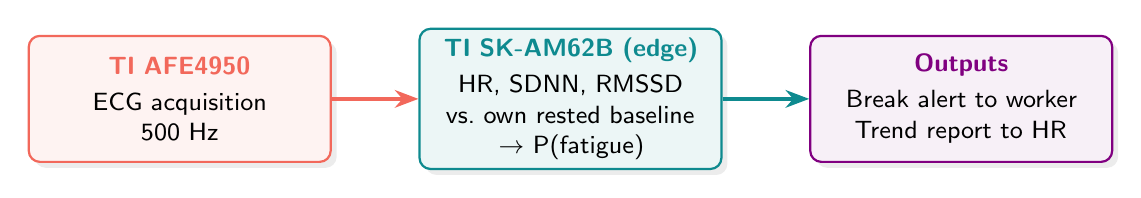
\begin{tikzpicture}[node distance=1.1cm, every node/.style={font=\sffamily\small},
  box/.style={rounded corners=4pt, align=center, minimum height=1.6cm, text width=3.6cm, thick, drop shadow={opacity=.15}}]
  \node[box, draw=bbcoral, fill=bbcoral!8] (afe) {\textbf{\color{bbcoral}TI AFE4950}\\[2pt]ECG acquisition\\500 Hz};
  \node[box, draw=bbteal, fill=bbteal!8, right=of afe] (edge) {\textbf{\color{bbteal}TI SK-AM62B (edge)}\\[2pt]HR, SDNN, RMSSD\\vs.\ own rested baseline\\$\rightarrow$ P(fatigue)};
  \node[box, draw=violet, fill=violet!6, right=of edge] (out) {\textbf{\color{violet}Outputs}\\[2pt]Break alert to worker\\Trend report to HR};
  \draw[-{Stealth[length=3mm]}, very thick, bbcoral] (afe) -- (edge);
  \draw[-{Stealth[length=3mm]}, very thick, bbteal] (edge) -- (out);
\end{tikzpicture}
\caption{BreathBreak architecture. Preprocessing, training and inference run on the edge board.}
\label{fig:arch}
\end{figure}

The AFE4950 \cite{afe4950} acquires the ECG. The SK-AM62B \cite{am62x} preprocesses the signal, extracts
heart-rate and HRV features, compares them with the wearer's own rested baseline, and produces a fatigue
probability (Figure~\ref{fig:arch}). In operation, each worker records a short rested baseline once.
Each subsequent recording or window is classified as \emph{normal}, \emph{watch} or \emph{fatigue}, and a
break is suggested only for sustained fatigue to avoid false alarms.

\subsection{Dataset}

We recorded ECG sessions with the AFE4950 evaluation module, each labeled \emph{normal} (rested) or
\emph{fatigue} by the participant. Because some sessions were contributed without a reliable subject label,
we assigned recordings to subjects by comparing their median heartbeat templates. Recordings of the same
subject correlate at 0.98--1.00, while recordings of different subjects correlate at 0.89--0.94. This yields
two subjects, A and C (Table~\ref{tab:data}).

\begin{table}[h]
\centering
\caption{Recordings used for modeling. Windows: 20-s windows (10-s step) with at least 12 clean beats.}
\label{tab:data}
\rowband\begin{tabular}{llrrrr}
\toprule
Subject & Condition & Recording & Duration (s) & Mean HR (bpm) & Windows \\
\midrule
A & rest    & 1 & 139.5 & 65 & 12 \\
A & rest    & 2 & 132.9 & 69 & 11 \\
A & fatigue & 1 &  27.6 & 107 & 1 \\
A & fatigue & 2 &  32.9 & 105 & 1 \\
A & fatigue & 3 &  37.7 & 108 & 2 \\
A & fatigue & 4 &  35.1 & 107 & 2 \\
A & fatigue & 5 &  31.1 &  94 & 1 \\
\midrule
C & rest    & 6 &  57.5 & 70 &  4 \\
C & rest    & 7 & 235.4 & 69 & 22 \\
C & rest    & 8 & 217.5 & 88 & 20 \\
C & fatigue & 6 & 152.4 & 106 & 13 \\
\bottomrule
\end{tabular}
\end{table}

\paragraph{Excluded recordings.}
Three further sessions of subject A were labeled \emph{normal} but had a mean HR of 105--109~bpm and
RMSSD of 7--20~ms, physiologically indistinguishable from the subject's fatigue sessions, so they were
evidently not recorded at rest. We excluded them from training and the rested baseline, and analyze them
separately in Section~\ref{sec:unrested}. One further recording was excluded because 25\% of it was
masked as motion artifact and its beat morphology matched no other recording.

\subsection{Preprocessing}

ECG is sampled at $f_s = 500$~Hz. Each recording is processed as follows:
\begin{enumerate}
  \item \textbf{Filtering.} DC removal, a 0.5~Hz high-pass filter (baseline wander), a 60~Hz notch
  (power-line interference) and a 40~Hz low-pass filter (muscle noise). All filters are zero-phase
  (forward--backward), so R-peak timing is not shifted.
  \item \textbf{Artifact masking.} One-second segments whose peak exceeds twice the typical peak
  (motion spikes), or where the raw signal saturates, are masked together with a $\pm$1-s margin.
  \item \textbf{R-peak detection.} Pan--Tompkins \cite{pantompkins1985}: a 5--20~Hz band-pass filter,
  derivative, squaring, 120~ms moving-window integration, and peak picking with a 330~ms minimum spacing
  and an adaptive height threshold. Each peak is then refined to the local maximum of the filtered ECG with
  automatic polarity detection. Peaks with amplitudes outside 0.5--1.6$\times$ the median are rejected.
  \item \textbf{RR cleaning.} RR intervals outside 0.33--1.5~s (40--180~bpm), intervals touching a masked
  segment, and intervals differing by more than 20\% from the local 5-beat median are rejected.
  \item \textbf{Stable range.} At least 2~s are trimmed from each end, and trimming continues while
  baseline drift or R-amplitude is unstable (electrode settling).
\end{enumerate}

\subsection{Features}
From the clean RR series we compute mean HR, SDNN, RMSSD, pNN50 and the HR range. From the median beat
template ($-200$ to $+400$~ms around each R-peak) we compute R-peak amplitude, T-to-R amplitude ratio and
the R-to-T interval:
\begin{equation}
\mathrm{SDNN} = \sqrt{\tfrac{1}{N-1}\textstyle\sum_{i}\left(RR_i-\overline{RR}\right)^2},\qquad
\mathrm{RMSSD} = \sqrt{\tfrac{1}{N-1}\textstyle\sum_{i}\left(RR_{i+1}-RR_i\right)^2}.
\end{equation}

\subsection{Personal-shift model}
\label{sec:shift}
Rather than classifying absolute feature values, we classify the \emph{change} from the wearer's own
rested baseline. For a new recording $x$ and a baseline recording $b$ of the same person we form
\begin{equation}
\Delta(x,b) = \left[\ln\frac{\mathrm{HR}_x}{\mathrm{HR}_b},\;
\ln\frac{\mathrm{SDNN}_x}{\mathrm{SDNN}_b},\;
\ln\frac{\mathrm{RMSSD}_x}{\mathrm{RMSSD}_b}\right],
\end{equation}
i.e.\ the percent change of each feature on a log scale. Percent changes make subjects with different
resting levels comparable. A log ratio of $0.4$ means about $+49\%$, whatever the person's baseline.

\paragraph{Training pairs.} For every subject we build:
\begin{itemize}
  \item \emph{fatigue pairs} ($y=1$): each fatigue recording against each of the subject's rested recordings;
  \item \emph{no-change pairs} ($y=0$): each rested recording against every other rested recording of the
  same subject, and the second half against the first half of every rested recording with at least 40~s
  of stable signal (and vice versa).
\end{itemize}
This gives 13 fatigue pairs and 18 no-change pairs.

\paragraph{Classifier: logistic regression.}
The classifier is a logistic regression on the three shift features. Each component of $\Delta$ is first
standardized with the mean $\mu_j$ and standard deviation $s_j$ of the training pairs,
$z_j = (\Delta_j-\mu_j)/s_j$, and the probability of fatigue is
\begin{equation}
P(\text{fatigue}\mid\Delta) = \sigma\!\left(w_{\mathrm{HR}}\,z_{\mathrm{HR}} + w_{\mathrm{SDNN}}\,z_{\mathrm{SDNN}}
+ w_{\mathrm{RMSSD}}\,z_{\mathrm{RMSSD}} + b\right),\qquad \sigma(u)=\frac{1}{1+e^{-u}} .
\end{equation}
The four parameters $(w_{\mathrm{HR}}, w_{\mathrm{SDNN}}, w_{\mathrm{RMSSD}}, b)$ minimize the class-balanced
cross-entropy loss with an L2 penalty ($\lambda=1$, intercept not penalized):
\begin{equation}
\mathcal{L}(\mathbf{w},b) = -\sum_{i} c_{y_i}\Big[y_i\ln p_i + (1-y_i)\ln(1-p_i)\Big] + \frac{\lambda}{2}\lVert\mathbf{w}\rVert^2,
\qquad c_{y} = \frac{N}{2N_{y}},
\end{equation}
where $N_y$ is the number of pairs in class $y$, so that fatigue and no-change pairs carry equal total weight.
The loss is convex and is minimized by Newton's method (iteratively reweighted least squares), which
converges in a few iterations and requires only matrix products and a $4\times4$ linear solve. This makes it
trivial to train on the board. On the board the model is implemented in pure NumPy (\texttt{board\_shift.py});
the laptop dashboard uses the equivalent scikit-learn \texttt{LogisticRegression}.

We deliberately chose a linear model with three physiologically motivated features. With 11 recordings, a
more flexible model (e.g.\ a neural network or tree ensemble) would have far more parameters than independent
examples and would memorize the training set. The signs of the learned weights can also be checked against
physiology: a positive weight on HR and negative weights on SDNN and RMSSD are expected
(Table~\ref{tab:weights}).

\paragraph{Decision.}
A new recording is compared with every baseline recording of that person, and the probabilities are averaged.
The output is \emph{fatigue} if $P\ge\tau$, \emph{watch} if $0.5\le P<\tau$, and \emph{normal} otherwise. The
alarm threshold $\tau$ is set just above the highest held-out score of a rested recording ($+0.05$, limited to
$[0.6, 0.9]$), so that rested sessions do not raise alarms. With our data, $\tau=0.6$.

\paragraph{Evaluation.}
\begin{itemize}
  \item \textbf{Leave-one-recording-out (LORO):} each recording is removed, the model is retrained on the
  rest, and the held-out recording is scored against the remaining rested recordings of the same subject.
  \item \textbf{Cross-subject transfer:} the model is trained on all windows of one subject and tested on
  every recording of the other subject, with no data from the test subject used in training.
\end{itemize}

\subsection{Transfer learning (Model B)}
\label{sec:modelb}
Our pitch also proposed a transfer-learning model: pre-train on a large public dataset, fine-tune, then
apply to our recordings. We implemented it with the same shift features, so the comparison isolates the
effect of the extra data:
\begin{itemize}
  \item \textbf{Pre-training on WESAD} \cite{wesad2018}: chest ECG (700~Hz) of 15 people, baseline vs.\
  Trier Social Stress Test. 60-s windows give 160 stress pairs and 160 no-change pairs.
  \item \textbf{Fine-tuning on DROZY} \cite{drozy2016}: ECG (512~Hz) recorded during three 10-minute sessions
  of increasing sleep deprivation, rated with the KSS \cite{kss1990}. Session 1 is the baseline and sessions with
  KSS~$\geq7$ are labeled sleepy (10 of 14 subjects had usable baseline ECG), giving 97 sleepy and 128 no-change pairs.
  \item \textbf{Fine-tuning on our data}: the same pairs as in Section~\ref{sec:shift}.
\end{itemize}
All signals are resampled to 500~Hz and processed with our pipeline. Fine-tuning is implemented as an L2
penalty that pulls the weights towards the previous stage's weights ($\lambda_{\text{prior}}\in\{0.01,0.1\}$).
As drawn in our slides, we also trained a small neural network (3--8--1, tanh). Its hidden layer was
pre-trained on WESAD and frozen, and only the output layer was re-trained on DROZY and then on our data.
Models are compared on our 11 recordings with the same leave-one-recording-out protocol, reporting accuracy,
the Brier score (mean squared error of the probability; lower is better) and the worst margin (the
smallest distance of any recording from the 0.5 decision boundary on the correct side).

\subsection{Windowing for long recordings}
For continuous monitoring, a long recording is cut into windows of the \emph{same} length used to compute
the baseline features, each window is scored, and the scores are aggregated (mean probability, or a
sustained rule such as three consecutive fatigued windows).

\subsection{Edge deployment on the SK-AM62B}
The board runs Linux with Python~3.14 and NumPy~2.4, but has no SciPy or pandas, no Wi-Fi and no network
cable. We therefore:
\begin{itemize}
  \item re-implemented zero-phase filtering (\texttt{filtfilt}, \texttt{lfilter\_zi}) and peak picking
  (\texttt{find\_peaks}) in NumPy with precomputed filter coefficients. The board pipeline matches the SciPy
  reference to within $10^{-13}$.
  \item wrote \texttt{board\_shift.py}, a single NumPy-only program with \texttt{train}, \texttt{check}
  and \texttt{enroll} commands. It reads a manifest of recordings, preprocesses them, trains the
  personal-shift model, runs the LORO evaluation and stores each subject's baseline in a JSON model file
  of a few kilobytes. Training the full dataset takes about 10~s on a laptop.
  \item transferred code and data over the 115{,}200-baud UART console in base64 chunks, each verified on the
  board by an MD5 checksum and re-sent if corrupted. Transfers resume after interruption.
\end{itemize}
A Streamlit dashboard on a laptop provides the user interface (baseline enrollment, checks, history and
HR reports) using the same model.

\subsection{Code availability}
The complete source code, recordings and setup instructions are available at
\url{https://github.com/nhattruong0205/HackEdge}. The README describes installation, dependencies
(NumPy only on the board; NumPy, SciPy, pandas, scikit-learn, Streamlit and Plotly on the laptop),
how to transfer the project to the SK-AM62B, how to train the model on the board
(\texttt{python3 board\_shift.py train}) and how to check a new recording
(\texttt{python3 board\_shift.py check A recording.csv}).

% =====================================================================
\section{Results and Discussion}

\subsection{Absolute features are dominated by the person}
Subjects A and C differ strongly in beat morphology: R-peak amplitude is 32~vs.\ 46~mV, and the T-wave
ratio and R-to-T interval also differ. Morphology also changes between sessions of the same subject as
electrode placement varies. In particular, the morphology features changed in \emph{opposite} directions in
the two subjects between rest and fatigue (Table~\ref{tab:shift}), so they cannot serve as fatigue markers.
A classifier on absolute features would mostly learn who is wearing the sensor.

\subsection{The rest-to-fatigue shift is large and consistent}

\begin{table}[h]
\centering
\caption{Rest vs.\ fatigue within each subject, using 20-s windows. $d$: Cohen's $d$; $p$: Mann--Whitney U.}
\label{tab:shift}
\rowband\begin{tabular}{l rrrr rrrr c}
\toprule
& \multicolumn{4}{c}{Subject A} & \multicolumn{4}{c}{Subject C} & Same \\
\cmidrule(lr){2-5}\cmidrule(lr){6-9}
Feature & Rest & Fatigue & $d$ & $p$ & Rest & Fatigue & $d$ & $p$ & direction \\
\midrule
HR (bpm)         & 67.1 & 105.6 & $+10.0$ & $10^{-6}$ & 77.5 & 106.0 & $+3.4$ & $10^{-7}$ & \textcolor{bbteal}{\checkmark} \\
SDNN (ms)        & 38.3 & 16.7  & $-2.8$  & $10^{-6}$ & 44.5 & 14.7  & $-2.2$ & $10^{-7}$ & \textcolor{bbteal}{\checkmark} \\
RMSSD (ms)       & 36.1 & 8.1   & $-6.3$  & $10^{-6}$ & 32.1 & 10.4  & $-2.6$ & $10^{-7}$ & \textcolor{bbteal}{\checkmark} \\
pNN50 (\%)       & 17.2 & 0.5   & $-2.4$  & $10^{-4}$ & 11.1 & 0.0   & $-1.8$ & $10^{-6}$ & \textcolor{bbteal}{\checkmark} \\
\midrule
R amplitude (mV) & 32.4 & 31.0  & $-0.7$  & 0.23      & 45.8 & 59.3  & $+4.1$ & $10^{-7}$ & \textcolor{bbcoral}{$\times$} \\
T/R ratio        & $-0.19$ & $-0.15$ & $+1.8$ & $10^{-5}$ & $-0.11$ & $-0.21$ & $-2.8$ & $10^{-7}$ & \textcolor{bbcoral}{$\times$} \\
\bottomrule
\end{tabular}
\end{table}

\begin{figure}[h]
\centering
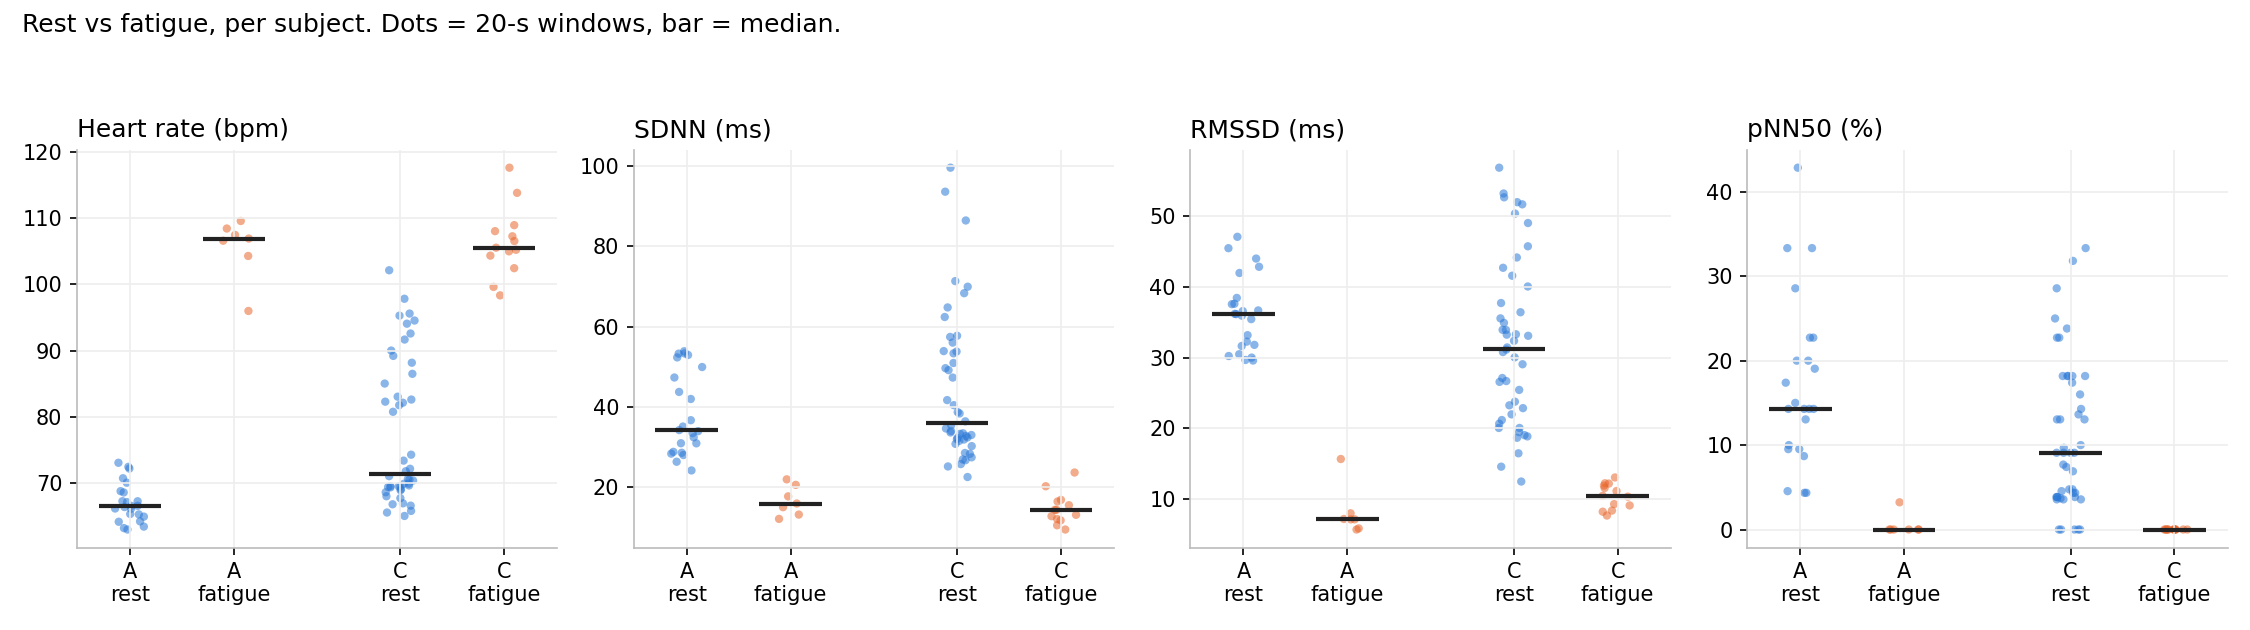
\includegraphics[width=\linewidth]{11_rest_vs_fatigue.png}
\caption{Heart rate and HRV at rest and in fatigue for both subjects. Both show the same shift:
HR up, SDNN, RMSSD and pNN50 down.}
\label{fig:shift}
\end{figure}

Table~\ref{tab:shift} and Figure~\ref{fig:shift} show that both subjects shift in the same direction on all
four HR/HRV features, with very large effects and $p<10^{-4}$. Relative to rest, HR increases by 58\% (A)
and 37\% (C), RMSSD falls by 78\% and 68\%, and SDNN by 56\% and 67\%. This is the classic signature of
reduced parasympathetic (vagal) and increased sympathetic activity \cite{taskforce1996,shaffer2017}.
In percent terms the two subjects are remarkably similar, even though their resting levels differ. This
motivates the percent-change features of Section~\ref{sec:shift}.

\subsection{Personal-shift model}

\begin{table}[h]
\centering
\caption{Leave-one-recording-out results of the personal-shift model (alarm threshold $\tau=0.6$).}
\label{tab:loro}
\rowband\begin{tabular}{llrl}
\toprule
Subject & Recording & $P(\text{fatigue})$ & Output \\
\midrule
A & rest 1    & 0.06 & normal \textcolor{bbteal}{\checkmark} \\
A & rest 2    & 0.09 & normal \textcolor{bbteal}{\checkmark} \\
A & fatigue 1 & 0.99 & fatigue \textcolor{bbteal}{\checkmark} \\
A & fatigue 2 & 1.00 & fatigue \textcolor{bbteal}{\checkmark} \\
A & fatigue 3 & 0.99 & fatigue \textcolor{bbteal}{\checkmark} \\
A & fatigue 4 & 0.98 & fatigue \textcolor{bbteal}{\checkmark} \\
A & fatigue 5 & 0.62 & fatigue \textcolor{bbteal}{\checkmark} \\
C & rest 6    & 0.14 & normal \textcolor{bbteal}{\checkmark} \\
C & rest 7    & 0.02 & normal \textcolor{bbteal}{\checkmark} \\
C & rest 8    & 0.25 & normal \textcolor{bbteal}{\checkmark} \\
C & fatigue 6 & 0.83 & fatigue \textcolor{bbteal}{\checkmark} \\
\midrule
\multicolumn{2}{l}{Total} & & 11/11 \\
\bottomrule
\end{tabular}
\end{table}

All 11 recordings are classified correctly (Table~\ref{tab:loro}), with no false alarms on rested
recordings. The learned weights (Table~\ref{tab:weights}) have the physiologically expected signs. HR has the
largest influence, followed by RMSSD. The weakest detection is fatigue recording 5 of subject A ($P=0.62$), which also had the smallest
HR increase (+43\%). The highest rested score is rest recording 8 of subject C ($P=0.25$), recorded at a
somewhat elevated HR of 88~bpm.

\begin{table}[h]
\centering
\caption{Learned logistic-regression parameters (trained on all 11 recordings), per standardized log-ratio.}
\label{tab:weights}
\rowband\begin{tabular}{lrl}
\toprule
Parameter & Value & Interpretation \\
\midrule
$w_{\mathrm{HR}}$    & $+1.49$ & higher HR than baseline $\rightarrow$ more likely fatigue \\
$w_{\mathrm{SDNN}}$  & $-0.85$ & lower SDNN than baseline $\rightarrow$ more likely fatigue \\
$w_{\mathrm{RMSSD}}$ & $-1.25$ & lower RMSSD than baseline $\rightarrow$ more likely fatigue \\
\bottomrule
\end{tabular}
\end{table}

\paragraph{Cross-subject transfer.}
Trained only on subject C and tested on subject A, the model classifies all 7 of A's recordings correctly
(rest: 0.08, 0.05; fatigue: 0.94, 0.97, 0.96, 0.89, 0.60). Trained only on subject A and tested on subject C,
it classifies all 4 of C's recordings correctly (rest: 0.12, 0.06, 0.31; fatigue: 0.83). The percent-change
representation was essential. When the same changes were instead standardized by each subject's own spread,
the model trained on A missed C's fatigue recording ($P=0.05$), because A's rested recordings vary much less
than C's.

\subsection{Does transfer learning help?}
\label{sec:modelb_res}

\begin{table}[h]
\centering
\caption{Transfer learning (Model B) vs.\ our model on our 11 recordings (leave-one-recording-out).
Brier: lower is better. Worst margin: negative means at least one recording is misclassified.}
\label{tab:modelb}
\rowband\begin{tabular}{lccc}
\toprule
Model & Correct & Brier & Worst margin \\
\midrule
\textbf{Ours only (logistic regression)}        & \textbf{11/11} & 0.025 & $+0.06$ \\
Zero-shot: WESAD                                 & 10/11 & 0.101 & $-0.38$ \\
Zero-shot: DROZY                                 & 9/11  & 0.159 & $-0.46$ \\
Zero-shot: WESAD $\rightarrow$ DROZY             & 9/11  & 0.147 & $-0.47$ \\
WESAD $\rightarrow$ DROZY $\rightarrow$ ours     & 10/11 & 0.035 & $-0.04$ \\
WESAD $\rightarrow$ ours                         & 11/11 & 0.028 & $+0.03$ \\
NN 3--8--1: WESAD $\rightarrow$ DROZY $\rightarrow$ ours (frozen) & 11/11 & 0.017 & $+0.11$ \\
NN 3--8--1: ours only                            & 11/11 & 0.020 & $+0.15$ \\
\bottomrule
\end{tabular}
\end{table}

Transfer learning did not improve on our model (Table~\ref{tab:modelb}). The full pipeline proposed in our
slides (WESAD $\rightarrow$ DROZY $\rightarrow$ ours) misclassified one rested recording, and no variant
exceeded 11/11. The frozen neural network had a slightly lower Brier score, but with 11 test recordings
this difference is within noise. In the cross-subject test (train on one subject, test on the other) our
model was also better calibrated (Brier 0.010 vs.\ 0.024). The source datasets explain why:
\begin{itemize}
  \item \textbf{WESAD stress} shifts in the same direction as our fatigue (HR $+34\%$, SDNN $-23\%$,
  RMSSD $-45\%$), so pre-training on it learns the right signs. However, it puts almost all weight on HR
  and flags our rested recording at 88~bpm (subject C, rest 8) as fatigued.
  \item \textbf{DROZY sleepiness} barely changes HR and HRV (HR $+5\%$, SDNN $+10\%$, RMSSD $-4\%$). Sleep
  deprivation in a quiet, seated task looks physiologically very different from our fatigue recordings
  (HR $+52\%$, RMSSD $-75\%$), so fine-tuning on it pulls the model in the wrong direction.
\end{itemize}
\paragraph{Logistic regression vs.\ transfer learning}
On our current data the personal-shift logistic regression is slightly better than every transfer-learning
variant: it is the only configuration that is both 11/11 correct and best calibrated in the cross-subject
test. It is also the simplest, with four parameters that train in seconds on the board and weights that
can be checked against physiology. The advantage is small, however. The best transfer model (the frozen
3--8--1 network) also classified all 11 recordings correctly. With only two subjects and 11 recordings,
none of these differences is statistically meaningful. We expect the balance to shift as data grow.
A logistic regression on three features can only learn ``HR up, HRV down''. Pre-training on large
public datasets can teach a richer model patterns that our small dataset cannot contain, such as how
HR and HRV respond to stress, exertion and sleepiness in many different people, and fine-tuning then
adapts it to our sensor and users. This benefit appears only when the source data resemble the target task. WESAD
helped in the right direction, while DROZY's sedentary sleepiness did not. With more of our own recordings,
and with a source dataset closer to occupational fatigue, we expect transfer learning to overtake the simple
model, especially for milder fatigue (Section~\ref{sec:heldout}). For deployment today, we keep the
personal-shift logistic regression.

\subsection{Held-out test recordings}
\label{sec:heldout}
After all models were fixed, we recorded one new rested and one new fatigued session that no model had
seen. Their beat templates match subject C (correlation 0.98--0.99), so both were scored against subject
C's rested baseline (Table~\ref{tab:heldout}).

\begin{table}[h]
\centering
\caption{New, unseen recordings of subject C. Change relative to C's rested baseline; $P$ = P(fatigue).}
\label{tab:heldout}
\rowband\begin{tabular}{lccccc}
\toprule
Recording & $\Delta$HR & $\Delta$SDNN & $\Delta$RMSSD & $P$ ours & $P$ transfer (W$\rightarrow$D$\rightarrow$ours) \\
\midrule
New rest    & $+1\%$  & $-18\%$ & $+20\%$ & 0.07 \textcolor{bbteal}{\checkmark} & 0.02 \textcolor{bbteal}{\checkmark} \\
New fatigue & $+16\%$ & $-42\%$ & $-38\%$ & 0.44 \textcolor{bbcoral}{$\times$} & 0.34 \textcolor{bbcoral}{$\times$} \\
\bottomrule
\end{tabular}
\end{table}

Both models correctly leave the new rested recording alone, but both miss the new fatigue recording.
Its shift points in the right direction (HR $+16\%$, SDNN $-42\%$, RMSSD $-38\%$) but is much milder than in the
training fatigue sessions (HR $+52\%$, RMSSD $-75\%$), so the probabilities stay just below 0.5. Scoring it
against the rested recording from the same session gives the same result ($P=0.45$). This is the most
important limitation revealed by the study. The model has only seen strong fatigue and does not yet detect
mild fatigue. Every other transfer variant also scored this recording between 0.34 and 0.48. Recording more mild-fatigue
sessions, and possibly lowering the \emph{watch} threshold, are the first next steps.

\subsection{Recordings labeled ``normal'' that were not at rest}
\label{sec:unrested}
The three excluded sessions of subject A, labeled normal but with HR of 105--109~bpm, score
$P=0.85$--$0.98$ against the subject's rested baseline. Physiologically they match the fatigue sessions
(beat-template correlation 0.99--1.00, RMSSD 7--20~ms). This illustrates the main practical risk of a
baseline-relative system. The baseline must be recorded genuinely at rest; a baseline recorded in an activated state
hides subsequent fatigue. Our app therefore warns when a baseline has HR above 90~bpm.

\subsection{Window length: train short, test long}
\label{sec:window}

\begin{table}[h]
\centering
\caption{Rest recording 1 of subject A (136~s): mean of 20-s window features vs.\ the whole recording.}
\label{tab:window}
\rowband\begin{tabular}{lrr}
\toprule
Feature & Mean of 20-s windows & Whole 136~s \\
\midrule
HR (bpm)       & 65.1 & 65.1 \\
HR range (bpm) & 9.4  & 15.5 \\
SDNN (ms)      & 34.3 & 38.9 \\
RMSSD (ms)     & 38.3 & 38.6 \\
pNN50 (\%)     & 22.1 & 21.2 \\
\bottomrule
\end{tabular}
\end{table}

HR, RMSSD and pNN50 are nearly independent of window length, but HR range (+65\%) and SDNN (+13\%) grow with
the window (Table~\ref{tab:window}), consistent with \cite{shaffer2017}. Baseline and test features must
therefore be computed over windows of equal length. A long recording is cut into such windows, each is
scored, and the scores are aggregated.

\subsection{Limitations}
\begin{itemize}
  \item \textbf{Mild fatigue.} A new, unseen mild-fatigue recording was missed by all models
  ($P=0.34$--$0.48$, Section~\ref{sec:heldout}).
  \item \textbf{Two subjects.} The cross-subject transfer is encouraging but rests on only two people and
  11 recordings. No population-level claim can be made.
  \item \textbf{Specificity.} The model detects sympathetic activation relative to rest. Subject C's fatigue
  recording shows HR falling steadily from about 122 to 98~bpm (Figure~\ref{fig:hr}), consistent with
  recovery after exertion. Exercise, stress or caffeine would produce a similar shift, so the model
  cannot yet distinguish fatigue from them.
  \item \textbf{Short recordings and labels.} Fatigue recordings of subject A are 28--38~s long, below the
  5-minute HRV standard \cite{taskforce1996}. Labels were self-reported without a KSS score.
  \item \textbf{PPG unused.} The optical channel was unavailable in about half of the recordings, so
  classification uses ECG only.
\end{itemize}

\begin{figure}[h]
\centering
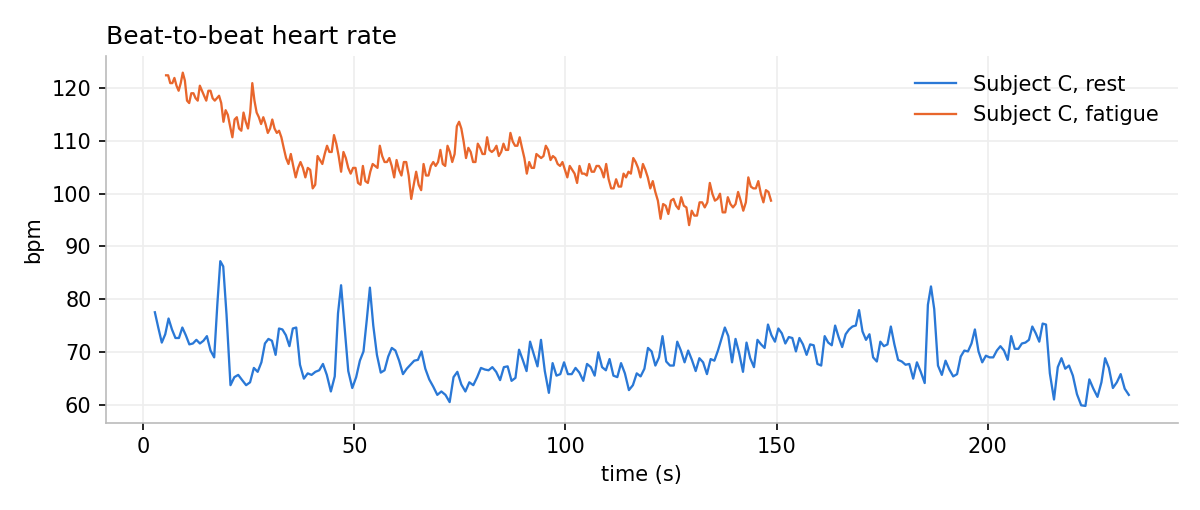
\includegraphics[width=0.75\linewidth]{12_subjectC_hr.png}
\caption{Beat-to-beat heart rate of subject C at rest and in the fatigue recording.}
\label{fig:hr}
\end{figure}

\subsection{Future work}
\begin{itemize}
  \item Record more subjects, each with paired rested and fatigued sessions of at least 3--5 minutes,
  labeled with KSS \cite{kss1990}. Rested sessions should follow 5 minutes of quiet sitting.
  \item Add features that separate fatigue from exertion and stress, e.g.\ ECG-derived respiration,
  PPG pulse arrival time, and the time course of HR over a shift.
  \item Use a source dataset closer to our setting (occupational fatigue recorded with a wearable ECG) for transfer learning; WESAD and DROZY did not help (Section~\ref{sec:modelb_res}).
  \item Stream AFE4950 data directly into the board for live, windowed alerts using the
  three-consecutive-windows rule.
\end{itemize}

\subsection{Conclusion}
Absolute ECG features mostly identify the person, but the change from a person's own rested state is
large and consistent: HR rises and SDNN, RMSSD and pNN50 fall. A three-feature personal-shift model built on
this observation classified all 11 of our recordings correctly, transferred between subjects in both
directions, and trains and runs on the TI SK-AM62B with NumPy alone. Larger, protocol-controlled studies
are needed to confirm the result and to distinguish fatigue from other causes of sympathetic activation.

% =====================================================================
\begin{thebibliography}{99}

\bibitem{williamson2000}
A.~M. Williamson and A.-M. Feyer, ``Moderate sleep deprivation produces impairments in cognitive and motor
performance equivalent to legally prescribed levels of alcohol intoxication,''
\emph{Occupational and Environmental Medicine}, vol.~57, no.~10, pp.~649--655, 2000.

\bibitem{taskforce1996}
Task Force of the European Society of Cardiology and the North American Society of Pacing and
Electrophysiology, ``Heart rate variability: Standards of measurement, physiological interpretation, and
clinical use,'' \emph{Circulation}, vol.~93, no.~5, pp.~1043--1065, 1996.

\bibitem{shaffer2017}
F.~Shaffer and J.~P. Ginsberg, ``An overview of heart rate variability metrics and norms,''
\emph{Frontiers in Public Health}, vol.~5, art.~258, 2017.

\bibitem{lal2001}
S.~K.~L. Lal and A.~Craig, ``A critical review of the psychophysiology of driver fatigue,''
\emph{Biological Psychology}, vol.~55, no.~3, pp.~173--194, 2001.

\bibitem{pantompkins1985}
J.~Pan and W.~J. Tompkins, ``A real-time QRS detection algorithm,''
\emph{IEEE Transactions on Biomedical Engineering}, vol.~BME-32, no.~3, pp.~230--236, 1985.

\bibitem{wesad2018}
P.~Schmidt, A.~Reiss, R.~Duerichen, C.~Marberger, and K.~Van~Laerhoven, ``Introducing WESAD, a multimodal
dataset for wearable stress and affect detection,'' in \emph{Proc.\ ACM International Conference on
Multimodal Interaction (ICMI)}, 2018, pp.~400--408.

\bibitem{drozy2016}
Q.~Massoz, T.~Langohr, C.~Fran\c{c}ois, and J.~G. Verly, ``The ULg multimodality drowsiness database
(called DROZY) and examples of use,'' in \emph{Proc.\ IEEE Winter Conference on Applications of Computer
Vision (WACV)}, 2016.

\bibitem{kss1990}
T.~{\AA}kerstedt and M.~Gillberg, ``Subjective and objective sleepiness in the active individual,''
\emph{International Journal of Neuroscience}, vol.~52, no.~1--2, pp.~29--37, 1990.

\bibitem{track1manual}
Texas Instruments / UTD HackEdge, ``Track~1: Edge Digital Twin for Continuous Physiological Monitoring ---
participant manual (AFE4950 and SK-AM62B),'' 2026.

\bibitem{afe4950}
Texas Instruments, ``AFE4950: Ultra-small, integrated AFE for wearable optical and ECG bio-sensing,''
product datasheet.

\bibitem{am62x}
Texas Instruments, ``SK-AM62B: AM62x starter kit for Arm Cortex-A53 based edge AI and HMI,'' user's guide.

\end{thebibliography}

\end{document}
